\chapter{The knowledge graph}
\label{chap:knowledge-graph}

  In this manual we define a \i{knowledge graph} as a collection of
  facts stated in a coherent way so that inferences can be drawn from
  them.  We implement a knowledge graph using the Resource Description
  Framework \citep{Lassila-99-RDF}, hereafter referred to as RDF.  The
  knowledge graph is the main value obtained from this project.

  The programs from chapter \refer{chap:command-line} read data in a
  domain-specific format, and translate it into \i{facts} in the form
  \triplet{subject}{predicate}{object}, which is the form of an RDF triplet.

  Once all desired data is described as RDF triplets, we can use the SPARQL
  Protocol and RDF Query Language \citep{sparql-11}, better known as simply
  ``SPARQL'', to extract knowledge from the facts.

\section{A layered inference system}

  Stating facts as RDF is a necessary first step to a more powerful inference
  system.  To understand the knowledge graph and its intended use, we can
  think of the knowledge graph as having multiple layers.  Figure
  \ref{fig:layered-knowledge} displays a small example of two layers.  The
  figure we shows knowledge from two separate sources (gene locations and
  genomic variants) from which we can derive new knowledge in an inference
  layer.

  \begin{figure}[H]
    \begin{center}
    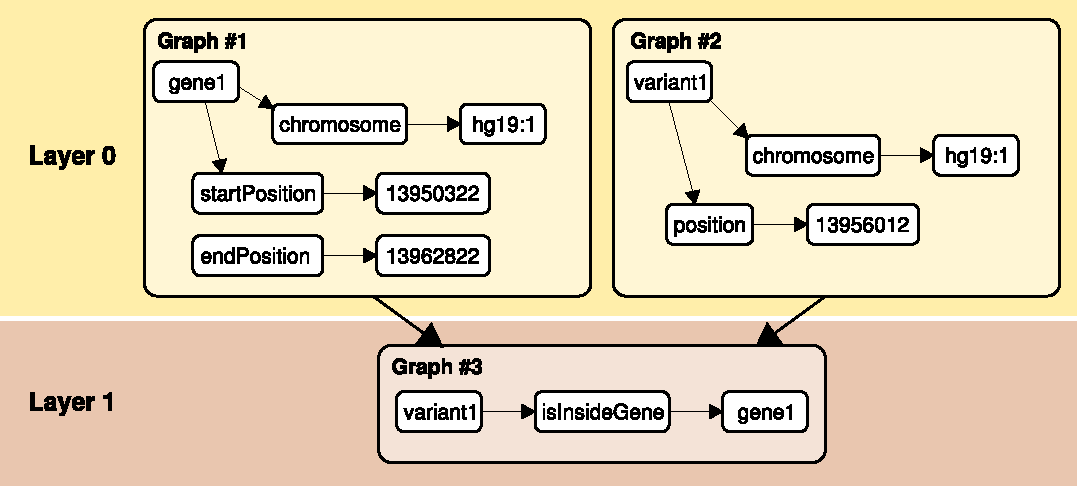
\includegraphics[width=1.0\textwidth]{figures/layered-knowledge.pdf}
    \end{center}
    \caption{\textit{An illustration of knowledge layers.}}
    \label{fig:layered-knowledge}
  \end{figure}

  Separating layers in graphs makes describing the flow of information easier,
  because the knowledge from a layer 1 graph can oftentimes be summarized as a
  query that described the relationship between the layer 0 graph(s) and the
  newly created layer 1 graph.

  Programs can operate on multiple layers of knowledge.  A program operates
  on the first layer (layer 0) when it translates a non-RDF format into RDF.
  These programs (re)state observations.  In the second layer (layer 1) and
  up, we find programs that operate on facts from layer 0 and generate
  inferences.

  From a computational perspective, these inferences allow programs to take
  shortcuts, and therefore answer questions (called \i{querying}) faster.
  The performance of querying the graph can therefore be tuned by cleverly
  stating facts.  For example, by using the inference drawn in figure
  \ref{fig:layered-knowledge}, a query asking for ``all variants in a gene''
  no longer needs to compute whether a variant is inside any of the
  genes.  The query planner can also narrow the search space by only
  considering the variants in the layer 1 graph.

  From a data access perspective, these inferences allow fine-grained access
  to knowledge.  For example, access to a layer 1 graph can be given, but
  not to its underlying layer 0 graph(s).  Properties can be removed (like
  patient identifiers), or made less precise (only tell that there is a
  variant in a particular gene, rather than the variant details).

  The knowledge graph contains two types of nodes; uniquely identifiable
  names having a symbolic value (1), and literal values like numbers and
  text (2).  Nodes with a symbolic value, or simply \i{symbols} can be used
  to add context to.  For example, consider the following statement:
  \triplet{<H>}{<electronegativity}{2.20}.  We can extend our knowledge
  about \code{<H>} by also stating: \triplet{<H>}{<numberOfElectrons>}{1}.
  The identifier \code{<H>} by itself has no meaning.  But that there is one
  ``thing'' for which both properties \code{<electronegativity>} and
  \code{<numberOfElectrons>} have a certain value provides insight into a
  deeper structure.

  \begin{sloppypar}
  We could go on and find more entities for which the properties
  \code{<electronegativity>} and \code{<numberOfElectrons>} are bound to
  specific values.  We can then identify the group of entities by a single
  \i{type} to make it easier to talk about.   In the example, the type
  \code{<ChemicalElement>} may be suitable.  So we would add the triplet:
  \triplet{<H>}{rdf:type}{<ChemicalElement>}.
  \end{sloppypar}
\section{Patterns for layer 0}

  The programs that are part of SPARQLing genomics use a few patterns to
  come up with identifiers.  For starters, the MD5 algorithm is used to come
  up with identifiers for the files that form the basis for layer 0.  We use
  a special URI prefix for these ``origins'':

  \ \ \ \ \triplet{<origin://d41d8cd98f00b204e9800998ecf8427e>}{rdf:type}
  {sg:Origin}

  By using a hashing algorithm we can safely assume that the identifiers will
  be the same when the input data was the same, regardless of who, when and
  in what order data was processed to (re)build the knowledge graph.

  This patterns is implemented by all programs described in chapter
  \refer{chap:command-line}.

\subsection{Public URIs and ontologies}
\label{sec:public-uris-and-ontologies}
  We have been using two types of symbols so far: internal (1) and publicly
  accessible (2).  We use the former for data-specific identifiers (like the
  MD5 sum for an origin) and the latter for increasing interoperability between
  distinct knowledge graphs.

  Such publicly accessible symbols are distributed in the form of a
  \i{vocabulary} or \i{ontology}.  In this manual the words ``vocabulary''
  and ``ontology'' are used interchangeably.  The use of symbols from various
  ontologies is the subject of chapter \refer{chap:implemented-ontologies}.
